% finalreport.tex - Final report for COSC 586

\documentclass{article}
\usepackage{times}
\usepackage{graphicx}
\usepackage{amsmath}
\usepackage{algorithm2e}
\usepackage[top=3cm, bottom=3cm, left=3cm, right=3cm]{geometry}

\begin{document}

\title{Predicting Change in a User's Mental State Based on Community Interaction in an Online Support Forum}
\author{
Julien Han\\
Tim Walsh\\
COSC 586\\
Georgetown University\\
}
\maketitle

\begin{abstract}
This paper proposes a new task related to the 2016 and 2017 CLPsych shared task, and presents a system that attempts to address the new task. Rather than directly classifying forum posts according to a user's apparent state of distress as previously done, this task involves predicting how a user's mental state will change based on their interaction with the forum community. The system first leverages another system that was successful in the original task to label the entire ReachOut.com dataset, and then uses a machine learning approach to predict the change in a target user's mental state based on replies by other forum users. The goal is to find correlation between how other users interact with a target user, and how the target user's distress increases or decreases, allowing us to learn how a community can better help forum users in distress.
\end{abstract}

\section{Introduction and Motivation}

\paragraph{}In 2016 and 2017, CLPsych challenged the text mining community to assist moderators of the online mental health support forum, ReachOut.com. Moderators wanted a way to automatically classify new posts (by applying $green$, $amber$, $red$, or $crisis$ labels) to quickly bring to their attention users in a state of distress who needed immediate support. CLPsych attracted 15 teams that submitted systems for this task, with top performing systems correctly labeling up to 95\% of the posts, and ReachOut.com now employs this technology on their forum\cite{milne}\cite{cohan2}.

\paragraph{}In trying to improve upon systems for this original task, based on previous research into peer influence and the "copycat suicide" effect, we hypothesized that higher and lower risk users may form social clusters and thus influence each other in more negative or positive ways\cite{gladwell}\cite{phillips}\cite{stack}. Concretely, this could involve building a social link graph based on conversations on the forum, computing risk scores for each user in a manner similar to the PageRank algorithm, and then including the user's score as another feature in the representation of their posts.

\paragraph{}From that intuition arose questions about how to confirm or deny the hypothesis. Successfully using it to improve results in the original task would provide some degree of confirmation, but we reasoned that we could measure influence more directly by defining a new task. The new task involves predicting how a user's mental state will change based on their interaction with other members of the forum community.

\paragraph{}Additionally, we hope to see if it is possible to predict changes in a user's mental state based on the activity of other forum users, then we can gain important insights from the trained model about how best help a forum user in distress. In particular, with a machine learning approach, extracting the most predictive features may teach us effective words and phrases to use, or topics to discuss, along with those we should avoid.

\section{Related Work}

\paragraph{}The 2016 CLPsych workshop proceedings present details and results from the work of 15 teams in the original task using the same ReachOut.com dataset. Every team used a machine learning approach with, at a minimum, bag-of-words features and a supervised learning method based the manually labeled subset of posts given for the task. Some teams incorporated a semi-supervised learning approach, leveraging datasets from Twitter and Reddit forums focused on depression. Teams selected many different combinations of features from the body text of each post as well as metadata associated with each post and user. Teams also used a variety of classifiers, with some in combination\cite{milne}. The top performing systems tended to focus on features from the body text, as opposed to metadata, such as token and character n-grams, part-of-speech tags, mood, sentiment, emotion, and topic. Top performing systems also used logistic regression and support vector machine classifiers. The highest performing system, by Kim et al, labeled the official test set with an F1 score of 0.42 and accuracy of 0.85\cite{kim}. Notably, some top performing systems included features from adjacent posts by other users. The intuition for this was to provide context, but it could also indicate influence.

\paragraph{}In follow-up work for the 2017 workshop, Cohan et al, improved their system to achieve an F1 score of 0.51 and accuracy of 0.95. Additionally, after labeling the entire dataset, Cohan et al used their results to explore other research questions. One discovery was that most users who were active for two or more months on the forum showed improvement in their apparent mental state as measured by the severity of their first and last posts: 81\% who began with a $crisis$ or $red$ post eventually posted content labeled $amber$ or $green$\cite{cohan2}. Cohan et al note that this may be due to a positive influence by the forum community.

\section{Approach}

\paragraph{}We first restructure and filter the dataset to produce "conversation sets." A conversation set consists of an original post or posts by a target user $U$ on day 0, followed by $L$ posts by other users that mention $U$ by-name over some period of $N$ days. Note that this is distinct from the concept of a forum "thread," which has one original post and subsequent replies that generally relate to one topic but may not directly address the original post or user. We then create a feature vector representation of the $L$ posts in the set, along with the label for $U$'s initial state and some additional metadata for the set. Finally, our classifier aims to predict the label of $U$'s next post appearing after the $N$-day period. In order to determine $U$'s initial state and train our classifer, we leverage the 2017 Cohan et al system to obtain labels for all posts in the dataset.

\paragraph{}For the parameter $N$, we experimented with values ranging from 1 to 14. At very low values of $N$, it is obvious that sets will contain few replies. In fact 40\% of sets contain no replies at $N$ = 1, but we did not remove those sets because getting no replies could have predictive power. Only 13\% of sets were empty at $N$ = 14. For large values of $N$, however, we believe that we begin to lose relevance. For example, it seems unlikely that something said on the forum in January would affect $U$'s state in December. Similarly, we also had to place a limit on the timing of $U$'s "next post," and we chose $N$ + 7. That is, if we did not find a "next post" to associate with a set within 7 days of the $N$-day period, we deleted that set. In addition to $N$-day periods, we also experimented with the idea of a "conversation snapshot" which looked at two consecutive posts by $U$, agnostic of time, and the replies occurring between those posts, but abandoned the idea after initial results were lower than conversation sets for all values of $N$.

\paragraph{}After constructing the sets, we filtered out all those sets where $U$ was a moderator. We did this because we are less interested in the mental state of moderators, and doing so helped to balance the training data since nearly all moderator posts are labeled $green$, both initially and finally. We also removed block-quotes written by $U$, and all occurrences of $U$'s username token in each set. These last two steps ensured that the classifier trained on the activity of other users instead of training on $U$ directly.

\paragraph{}We then extracted and experimented with the following features for each set: TF-IDF weighted unigrams, bigrams, and trigrams (stop words both included and removed using the NLTK list), the number of replies in the set, the number of replies by a moderator, the number of posts by $U$ during the $N$ day period, a simple average risk score for users replying to $U$, sentiment polarity, and sentiment subjectivity. We defined a risk score for a replying user as the percentage of their posts in the total dataset that were $flagged$. We determined polarity and subjectivity for all the replies lumped together using the TextBlob package. If a conversation set contained no replies, we set values for these last three features to be neutral, choosing 0.07 as a neutral risk score because 7\% of posts in the entire dataset are $flagged$.

\paragraph{}After building the feature vectors from the conversation set, we feed them to a classifier. The classifier that we chose was a support vector machine with linear kernel. We picked a linear kernel so that the coefficients of the trained model would correspond directly to the feature vector. That way we can extract the coefficients and see how each feature contributes to the decision. Specifically, the features will be words (unigrams), phrases (bigrams and trigrams), along other features mentioned above. The weight for the words and phrases indicate how strongly the words and phrases are related to each case where $U$ transitions from one state to another. 

\section{Experimental Setup}

\paragraph{}As we were defining this task ourselves, we had to reason about many details of the setup. The first detail was how many labels to use. To ensure the highest level of accuracy, we chose to use only $green$ and $flagged,$ where $amber$, $red$, and $crisis$ were lumped together as $flagged,$ because the Cohan et al system succeeded in this task with an F1 score 0.92. Another detail was determining the label for $U$'s initial state. If $U$ made just one post on day 0, we simply took the label of that post. In the case where $U$ made multiple posts on day 0, we tried three different methods. The "absolute" method set the initial state to be $flagged$ if any post on day 0 was $flagged$. The "last post" method took the label of the final post made by $U$ on day 0. The "majority" method set the initial state as $flagged$ if 50\% or more posts on day 0 were $flagged$. The "absolute" method produced twice as many $flagged$ cases, giving us the most balanced training data, and giving us the best initial results, so we performed all subsequent trials with this method. A third detail was determining how to define a "reply" to include in a conversation set. We used several different types of replies. One is when $U$ is quoted with the forum's block-quote functionality. The others are the appearance of patterns such as "Hey $U$, ..." or "...@$U$..." in the body text.

\paragraph{Dataset}The dataset provided by CLPsych for its 2016 shared task includes 65,755 posts from the ReachOut.com forum from July of 2012 to June of 2015. Labels for the entire dataset were provided by the 2017 Cohan et al system.

\paragraph{Evaluation Plan}We evaluated our system with 5-fold cross validation looking at F1 score, accuracy, precision, and recall. F1 score is what we present in this paper. We separately evaluated conversation sets with a $green$ initial state, sets with a $flagged$ initial state, and all sets together (with initial state label as a feature). Working separately on sets that only begin with a $flagged$ state, for example, lets us reason specifically about how distressed users are affected by the highest and lowest weight features in our analysis.

\paragraph{Results}We achieved our highest F1 score of 0.776 for all conversation sets at $N$ = 14, using the following features: TF-IDF unigrams and bigrams with stop words included, number of replies, and number of replies by a moderator. Adding all additional features (still including stop words) produced our next best F1 score of 0.775. We had our third best F1 score of 0.772 after removing stop words. In general, as $N$ ranged from 1 to 14, the F1 score ranged from about 0.65 to 0.77, but the increase was only monotonic up to about $N$ = 10, after which improvement flattened out. See Figure 1.

\begin{figure}[h!]
    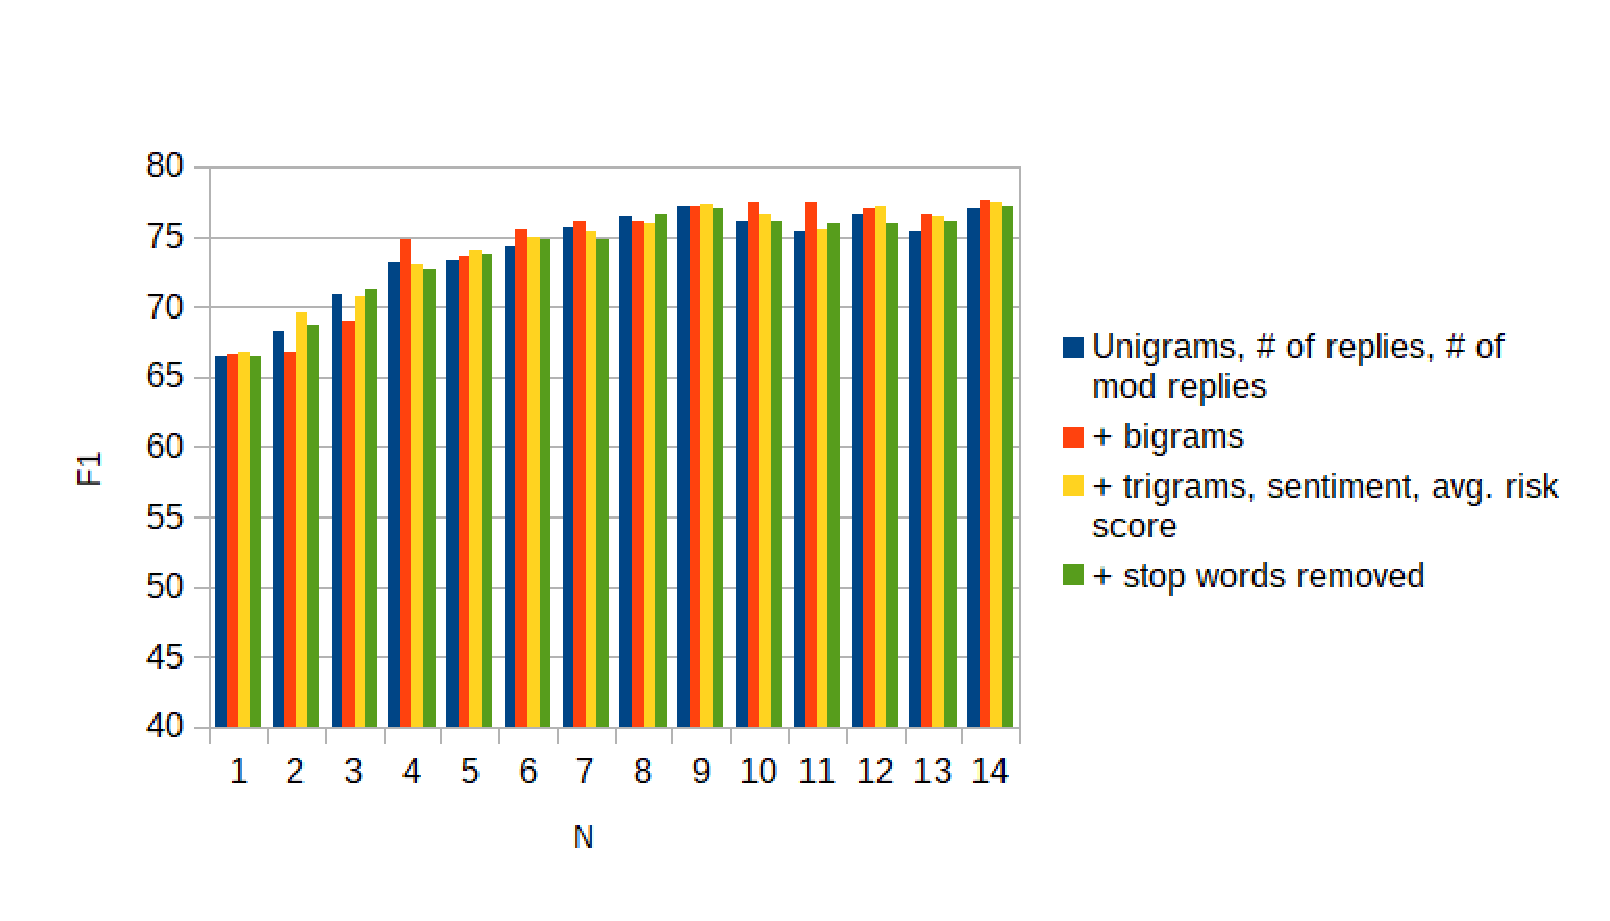
\includegraphics[width=14cm]{resultsAll}
    \caption{All Sets with Initial State Label as Feature}
\end{figure}

\subparagraph{}When the initial state was $flagged$, we achieved our highest F1 score of 0.771 at $N$ = 10, with all features and stop words included. See Figure 2.

\begin{figure}[h!]
    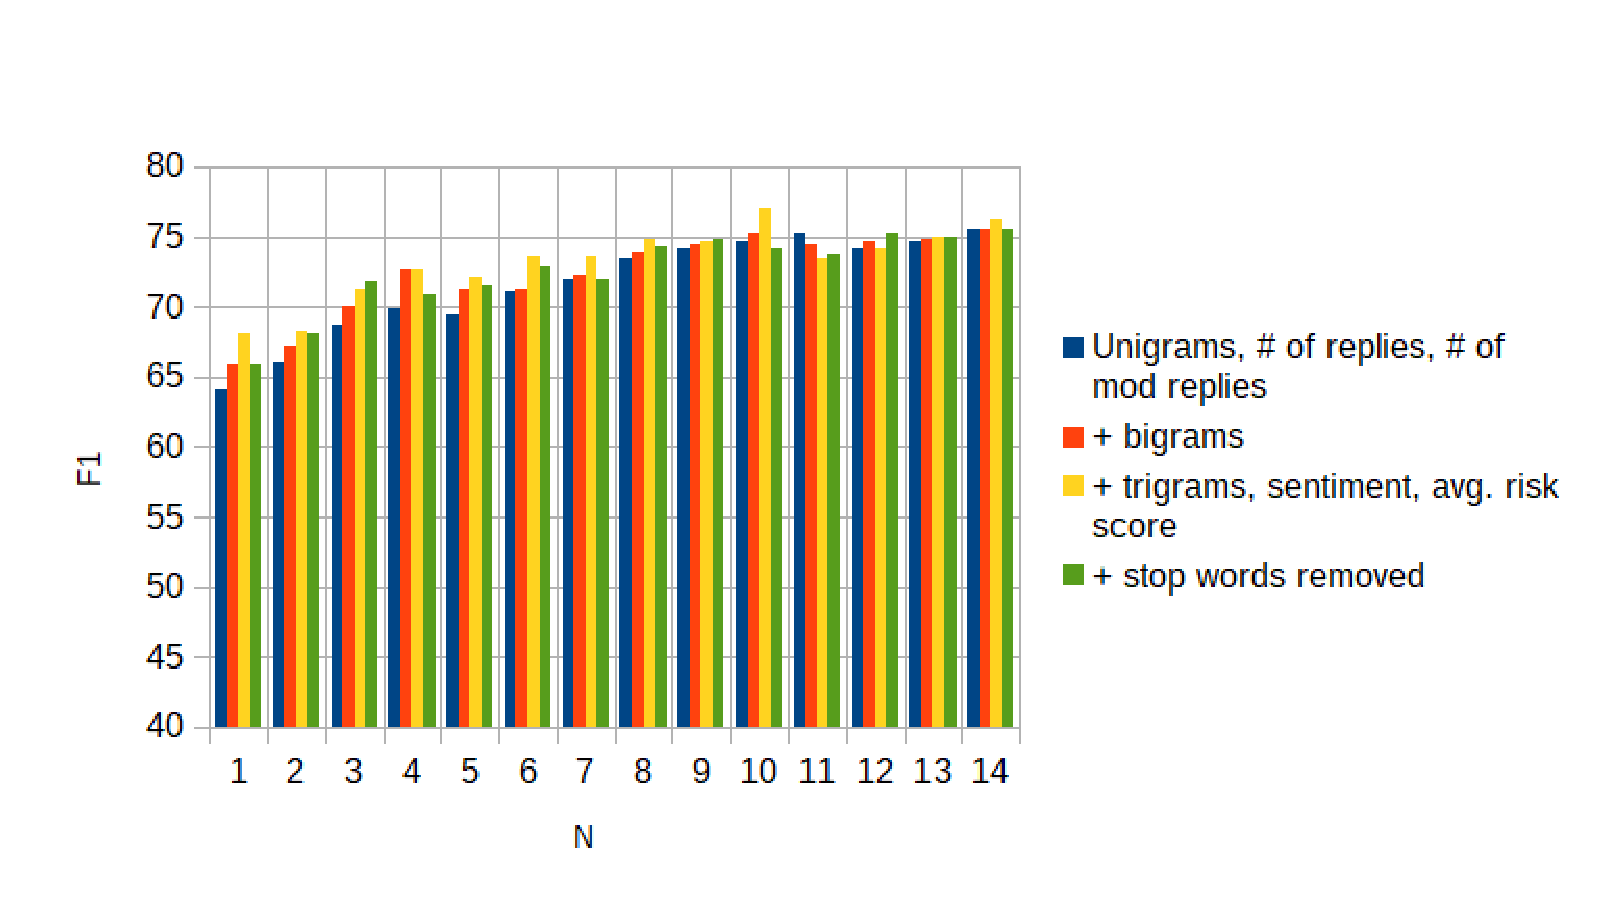
\includegraphics[width=14cm]{resultsFlagged}
    \caption{Sets with Flagged Initial State Only}
\end{figure}

\subparagraph{}When the initial state was $green$, we achieved our highest F1 score of 0.628 at $N$ = 14, with all features and stop words removed. The significantly lower score on these sets is likely explained by the extreme imbalance of the dataset. About 95\% of conversation sets with an initial state of $green$ stay $green$, compared to about 40\% of sets with an initial state of $flagged$ that stay $flagged$. In fact, before we removed conversation sets where $U$ was a moderator, the imbalance was so extreme that our classifier simply predicted $green$ for 100\% of these sets. See Figure 3.

\begin{figure}[h!]
    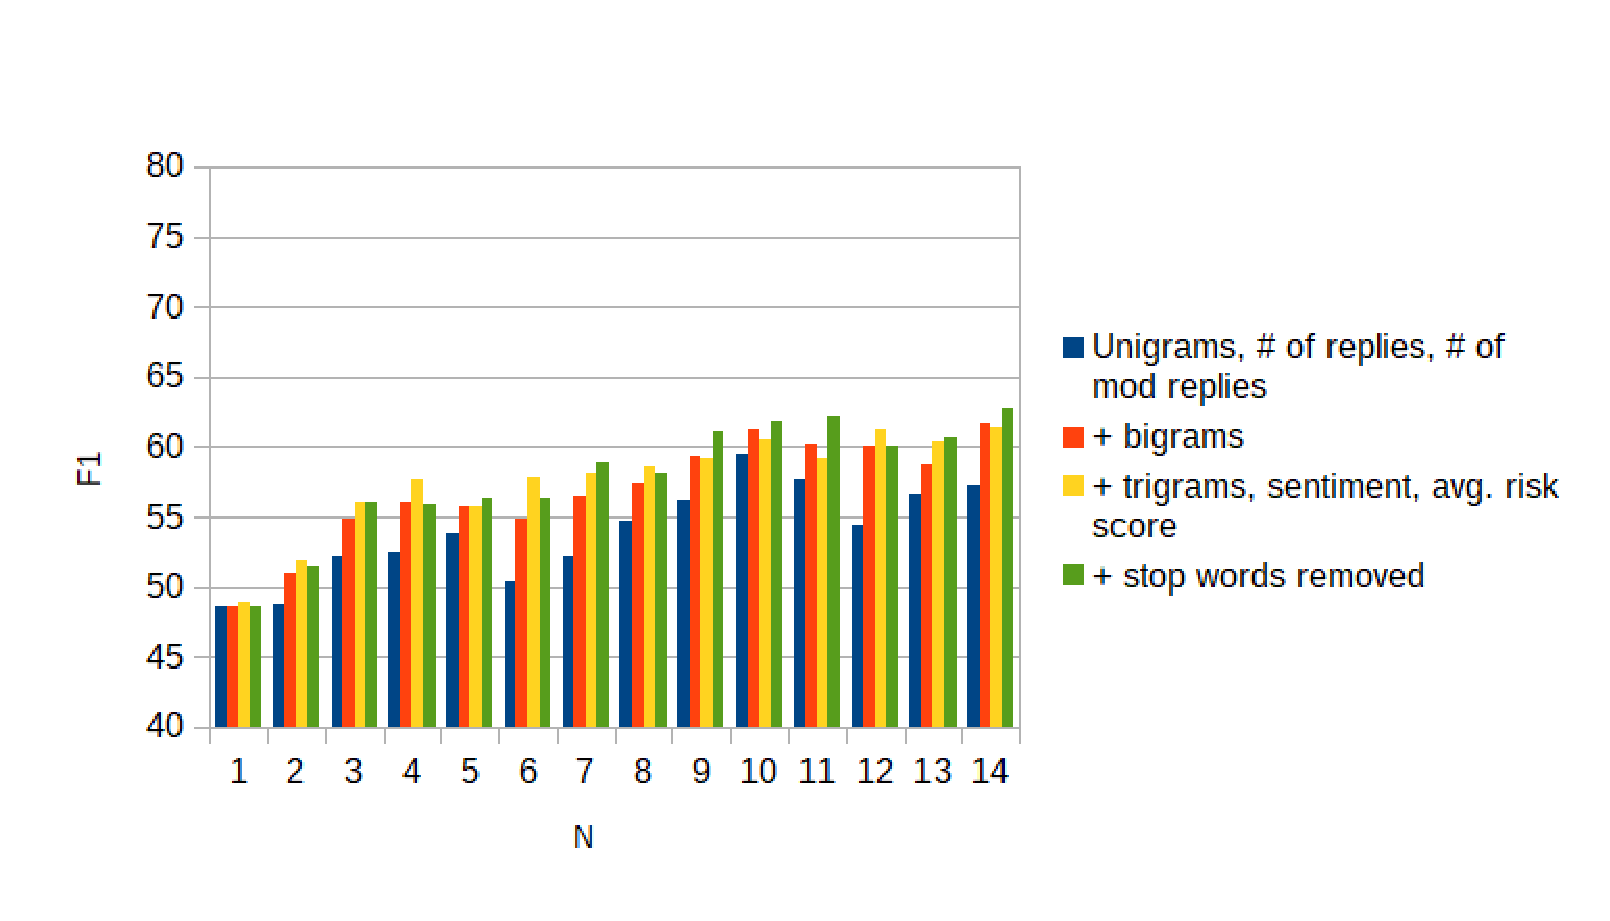
\includegraphics[width=14cm]{resultsGreen}
    \caption{Sets with Green Initial State Only}
\end{figure}

\subparagraph{}Once we had models that predict the change in $U$'s state reasonably well, we turned our attention to the follow-up question of how to interpret the model and gain insight into what factors might influence $U$'s level of distress and how. To achieve this, we extracted the top feature weights from each trained model. Here we examine the separate cases for each initial and final state label. In Figure 4, highlighted in red are (anonymized) usernames and custom features (as opposed to text N-grams). *norepliesfound* is a special token that we inserted into conversation sets when they were otherwise empty. Some features stand out for their peculiarity. One is "year 11" or "11" which refers to the 11th grade of school in Australia, for students of age 16 or 17. Another is "jaw" which showed up in a number of posts talking about TMJ pain, associated with grinding or clenching teeth.

\begin{figure}[h!]
    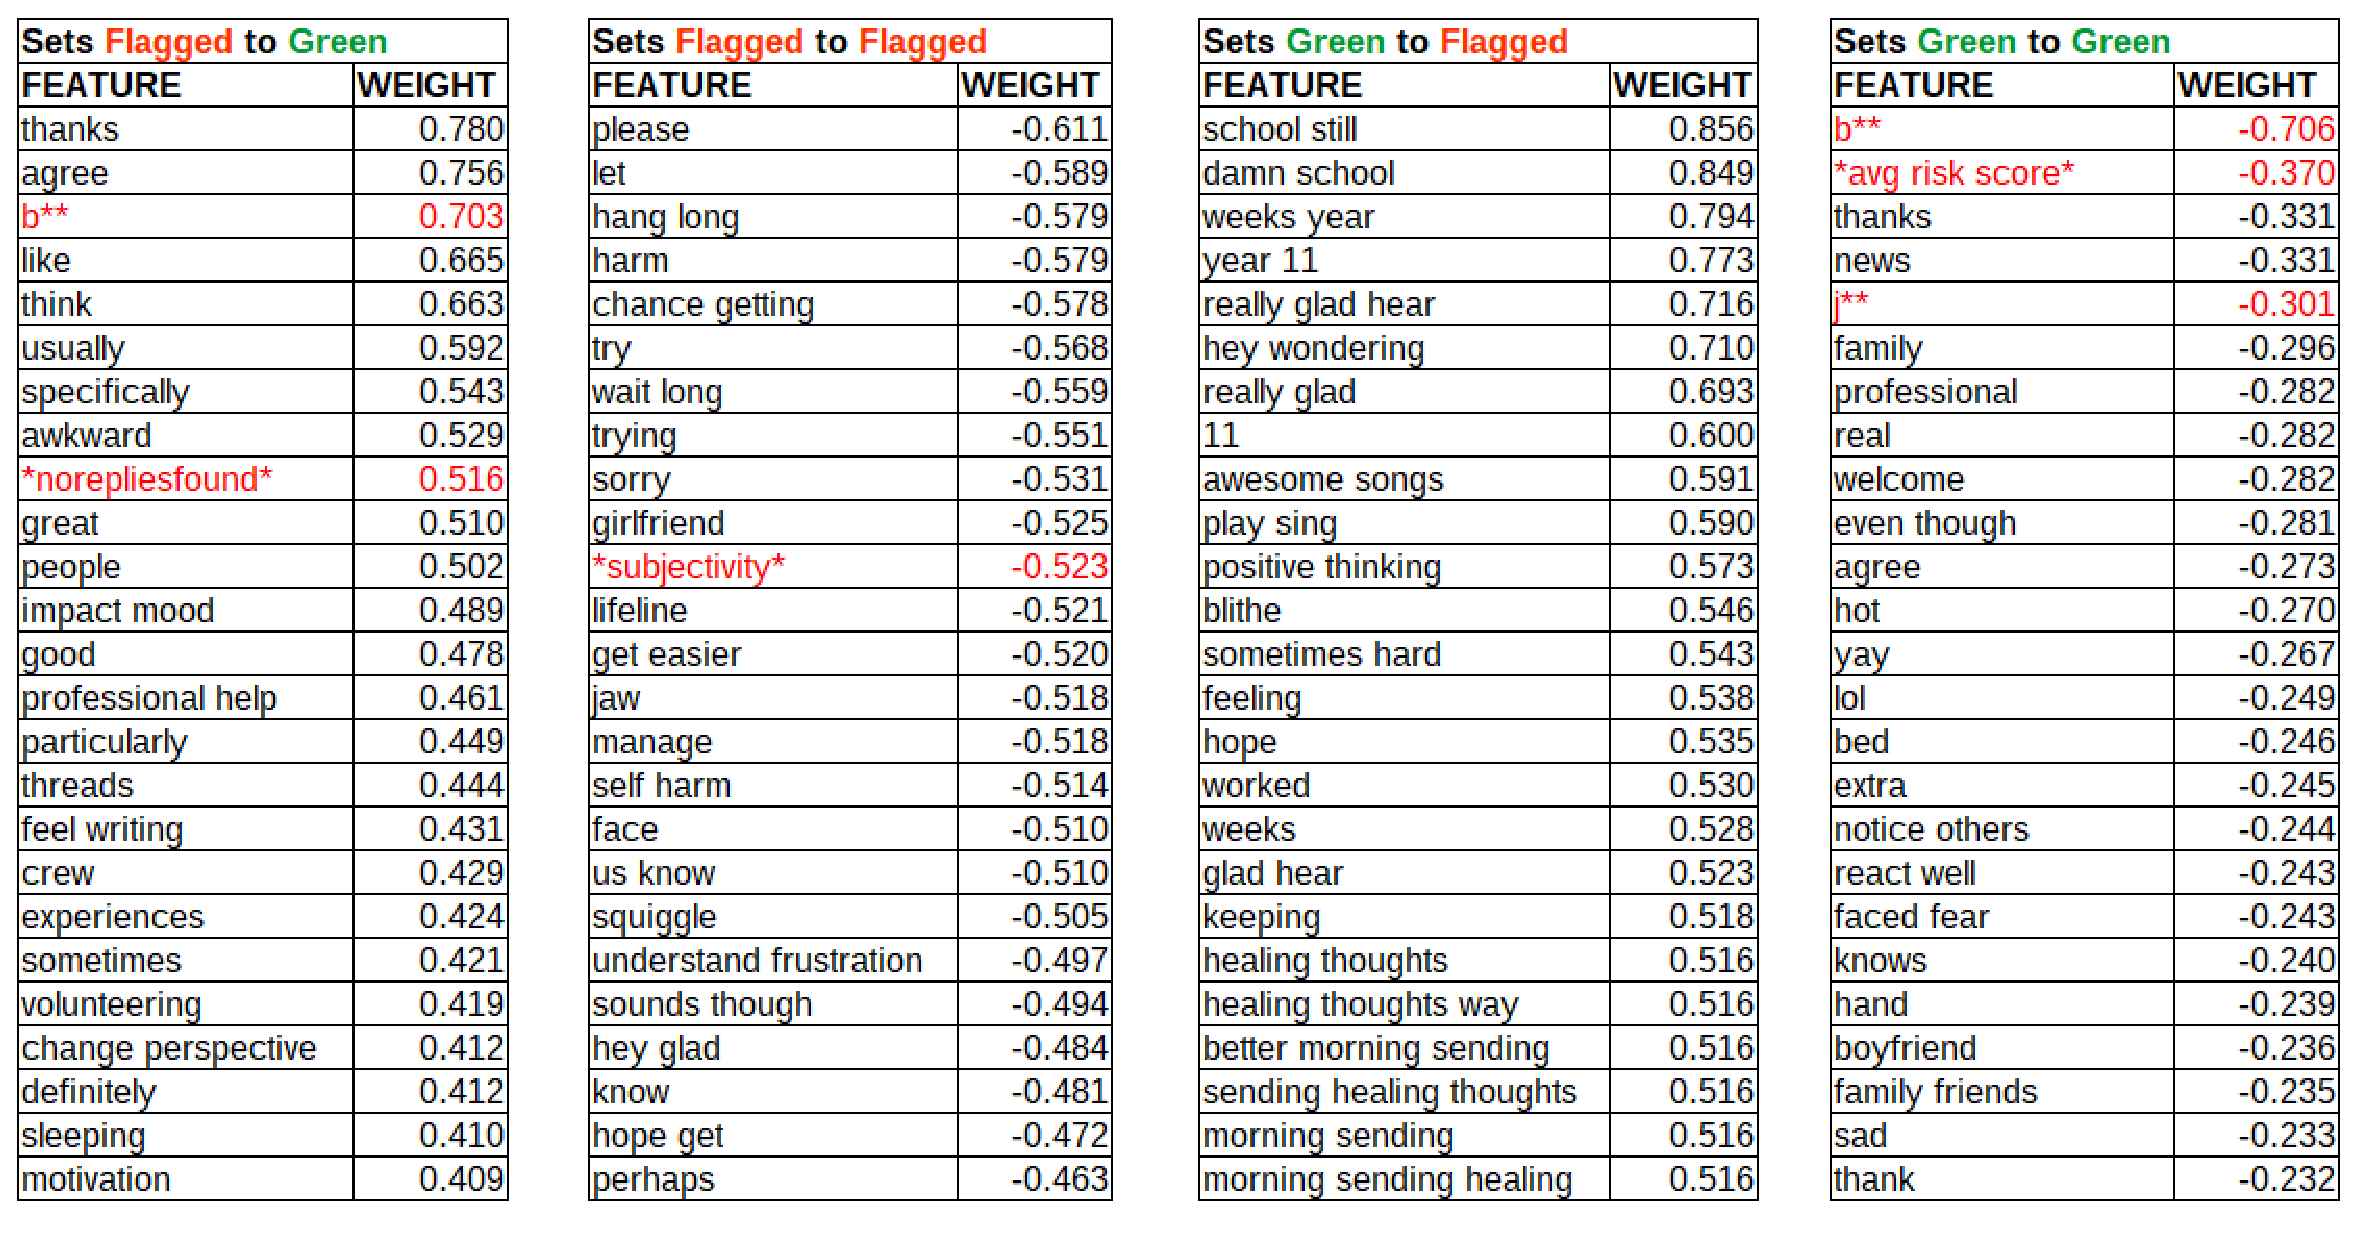
\includegraphics[width=16cm]{topfeatures}
    \caption{Highest/Lowest Weighted Features from Trained Models}
\end{figure}

\paragraph{Analysis}Our work on this task frequently generated new questions rather than answers, and we discuss the most significant remaining questions here.

\subparagraph{1. Are replies actually a factor that drive change in $U$'s state, or are they simply a reflection of $U$'s state?}We would like to be able to conclude that our top weighted features (for sets that move from a state of $flagged$ to $green$, for example) provide guidance to the ReachOut.com community about how to help a user in distress. The $flagged \rightarrow green$ top weighted terms receive a subjectivity score of 0.9 and positivity score of 0.9 using the NLTK sentiment analysis package, so they seem likely to influence $U$ in a positive way. The case with $flagged \rightarrow flagged$ top features is symmetical, having a polarity score of 0.9 and negativity score of 0.7. But causality is unclear, because the appearance of positive (or negative) language is also exactly what we would expect to see in a conversation involving a $U$ with a positive (negative) attitude whose mental state is becoming more positive (negative). The top weighted terms from $green \rightarrow flagged$ actually get a positivity score of 0.7, so it is difficult to argue that the replies caused $U$'s distress to increase. There are many other explanations for the change in $U$'s mental state. Offline events likely have more influence than discussions on the forum. Some people might also be affected by simply thinking and writing about their feelings, regardless of any replies written to them (supported by the fact that our *norepliesfound* token was predictive of a $flagged$ $U$ turning $green$). Or people could be affected by passively reading other content on the forum that was not directed to them at all.

\subparagraph{2. Are some users more positively or negatively influential than others, or do they simply choose to participate on the forum in different ways?}This is similar to first question. Some usernames show up in our top weighted terms lists, and we would like to be able to conclude that those users are especially influential, and that their style of writing could serve as a model for what other users should do or not do. However, it is equally likely that some users simply choose to interact only with users or threads that have a positive tone. Others might focus on trying to help people who are suffering the most. We note that the two users who appear in Figure 4 posted an above-average proportion of $flagged$ content (16-18\% vs. 7\% for the forum at large) despite appearing on the lists for $flagged \rightarrow green$ and $green \rightarrow green$.

\subparagraph{3. What is the effect of survivorship bias on our results?}It is important to note that we were able to construct only about 6,000 conversation sets for any value of $N$ (about 10,000 before removing the sets where $U$ was a moderator) when the dataset contained more than 65,000 posts. The difference is large because most of the time $U$ did not make a follow-up post, so we could not complete the set and add it to our training data. Therefore, we cannot conclude anything about these users who stopped participating on the forum, and they might be the majority of users.

\section{Conclusion}

\paragraph{}With the set of features and classifier described in this paper, we can predict the change in an active ReachOut.com user's apparent mental state based on replies by other users in the community. But there remains a lot of analysis and reasoning to be done before we can leverage the model to gain valuable insight into better helping users in distress. Specifically, we would like to see if there are certain words, phrases, or topics that bring a distressed user to a $green$ state, but the top terms we extracted do not show a strong pattern; some make intuitive sense but some do not. Moreover, reasoning about causation is very difficult. However, we believe that the ReachOut.com dataset remains valuable for this line of inquiry, and we hope that other researchers will take an interest and design better experiments to improve upon our results.

\begin{thebibliography}{9}

	\bibitem{milne}
	David N. Milne, Glen Pink, Ben Hachey, and Rafael A. Calvo. 2016. Clpsych 2016 shared task: Triaging content in online peer-support forums. In Proceedings of the Third Workshop on Computational Lingusitics and Clinical Psychology. Association for Computational Linguistics, San Diego, CA, USA, pages 106–117.
	\bibitem{kim}
	Sunghwan Mac Kim, Yufei Wang, Stephen Wan, and Cecile Paris. 2016. Data61-CSIRO systems at the CLPsych 2016 Shared Task. In Proceedings of the 3rd Workshop on Computational Linguistics and Clinical Psychology: From Linguistic Signal to Clinical Reality, San Diego, California, USA, June 16.
        \bibitem{cohan2}
        Cohan, Arman, Sydney Young, Andrew Yates, and Nazli Goharian. "Triaging Content Severity in Online Mental Health Forums." arXiv preprint arXiv:1702.06875 (2017).
        \bibitem{gladwell}
        Gladwell, Malcolm. The Tipping Point: How Little Things Can Make a Big Difference. New York: Little, Brown and Company Hachette Book Group, 2002. eBook Edition.
        \bibitem{phillips}
        Phillips, David. The Influence of Suggestion on Suicide: Substantive and Theoretical Implications of the Werther Effect. American Sociological Review Vol. 39, No. 3 (Jun., 1974), pp. 340-354
        \bibitem{stack}
        Stack, Steven. "Media coverage as a risk factor in suicide." Journal of Epidemiology \& Community Health 57.4 (2003): 238-240.

\end{thebibliography}

\end{document}
